\documentclass{standalone}
\usepackage{tikz}
\usetikzlibrary{patterns, positioning}

\begin{document}
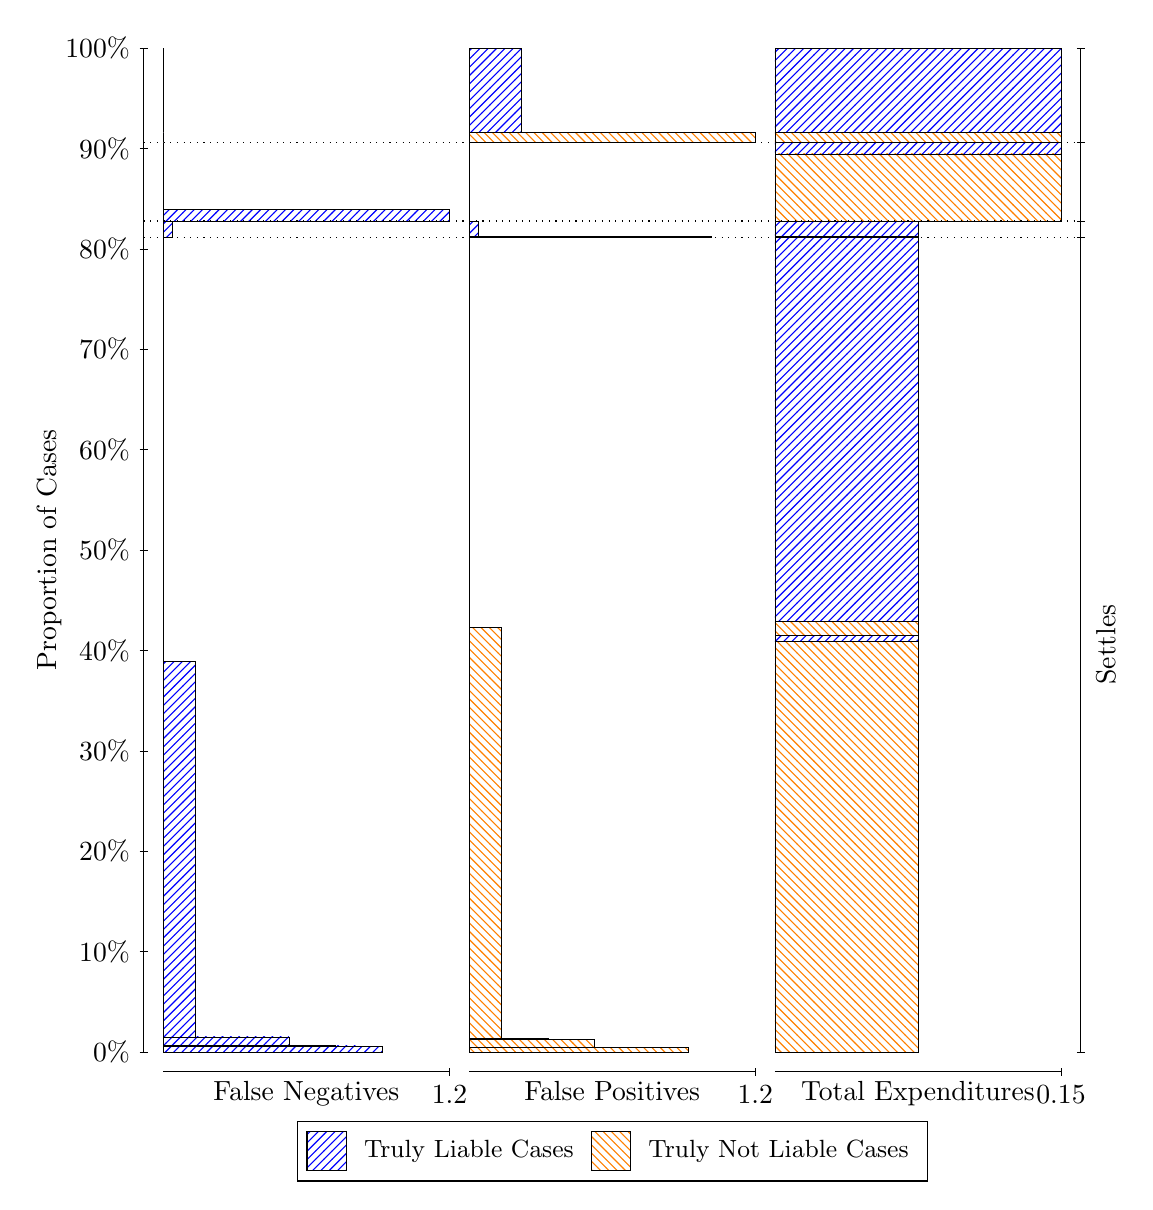
\begin{tikzpicture}
\draw[black, very thin] (1.5,1.75) -- (1.5,14.5);
\node[rotate=90, anchor=center] at (0.3, 8.125) {Proportion of Cases};
\draw[black, very thin] (1.45,1.75) -- (1.55,1.75);
\node[anchor=east] at (1.45, 1.75) {0\%};
\draw[black, very thin] (1.45,3.025) -- (1.55,3.025);
\node[anchor=east] at (1.45, 3.025) {10\%};
\draw[black, very thin] (1.45,4.3) -- (1.55,4.3);
\node[anchor=east] at (1.45, 4.3) {20\%};
\draw[black, very thin] (1.45,5.575) -- (1.55,5.575);
\node[anchor=east] at (1.45, 5.575) {30\%};
\draw[black, very thin] (1.45,6.85) -- (1.55,6.85);
\node[anchor=east] at (1.45, 6.85) {40\%};
\draw[black, very thin] (1.45,8.125) -- (1.55,8.125);
\node[anchor=east] at (1.45, 8.125) {50\%};
\draw[black, very thin] (1.45,9.4) -- (1.55,9.4);
\node[anchor=east] at (1.45, 9.4) {60\%};
\draw[black, very thin] (1.45,10.675) -- (1.55,10.675);
\node[anchor=east] at (1.45, 10.675) {70\%};
\draw[black, very thin] (1.45,11.95) -- (1.55,11.95);
\node[anchor=east] at (1.45, 11.95) {80\%};
\draw[black, very thin] (1.45,13.225) -- (1.55,13.225);
\node[anchor=east] at (1.45, 13.225) {90\%};
\draw[black, very thin] (1.45,14.5) -- (1.55,14.5);
\node[anchor=east] at (1.45, 14.5) {100\%};

\draw[black, very thin] (13.4,1.75) -- (13.4,14.5);
\draw[black, very thin] (13.35,1.75) -- (13.45,1.75);
\node[anchor=west] at (13.35, 1.75) {};
\draw[black, very thin] (13.35,12.098) -- (13.45,12.098);
\node[anchor=west] at (13.35, 12.098) {};
\draw[black, very thin] (13.35,12.303) -- (13.45,12.303);
\node[anchor=west] at (13.35, 12.303) {};
\draw[black, very thin] (13.35,13.3) -- (13.45,13.3);
\node[anchor=west] at (13.35, 13.3) {};
\draw[black, very thin] (13.35,14.5) -- (13.45,14.5);
\node[anchor=west] at (13.35, 14.5) {};

\draw[black, very thin, pattern color=blue, pattern=north east lines] (1.75,1.75) rectangle (4.5306,1.8238);
\draw[black, very thin, pattern color=blue, pattern=north east lines] (1.75,1.8238) rectangle (4.234,1.8271);
\draw[black, very thin, pattern color=blue, pattern=north east lines] (1.75,1.8271) rectangle (3.9374,1.8305);
\draw[black, very thin, pattern color=blue, pattern=north east lines] (1.75,1.8305) rectangle (3.6408,1.8341);
\draw[black, very thin, pattern color=blue, pattern=north east lines] (1.75,1.8341) rectangle (3.3442,1.9426);
\draw[black, very thin, pattern color=blue, pattern=north east lines] (1.75,1.9426) rectangle (2.1578,6.7104);
\draw[black, very thin, pattern color=orange, pattern=north west lines] (1.75,6.7104) rectangle (1.75,12.098);
\draw[black, very thin, pattern color=blue, pattern=north east lines] (1.75,12.098) rectangle (1.8612,12.297);
\draw[black, very thin, pattern color=orange, pattern=north west lines] (1.75,12.297) rectangle (1.75,12.303);
\draw[black, very thin, pattern color=blue, pattern=north east lines] (1.75,12.303) rectangle (5.3833,12.446);
\draw[black, very thin, pattern color=orange, pattern=north west lines] (1.75,12.446) rectangle (1.75,13.3);
\draw[black, very thin, pattern color=orange, pattern=north west lines] (1.75,13.3) rectangle (1.75,13.428);
\draw[black, very thin, pattern color=blue, pattern=north east lines] (1.75,13.428) rectangle (1.75,14.5);
\draw[black, very thin, pattern color=orange, pattern=north west lines] (5.6333,1.75) rectangle (8.4139,1.8087);
\draw[black, very thin, pattern color=orange, pattern=north west lines] (5.6333,1.8087) rectangle (7.2276,1.9087);
\draw[black, very thin, pattern color=orange, pattern=north west lines] (5.6333,1.9087) rectangle (6.931,1.9145);
\draw[black, very thin, pattern color=orange, pattern=north west lines] (5.6333,1.9145) rectangle (6.6344,1.9201);
\draw[black, very thin, pattern color=orange, pattern=north west lines] (5.6333,1.9201) rectangle (6.3378,1.9255);
\draw[black, very thin, pattern color=orange, pattern=north west lines] (5.6333,1.9255) rectangle (6.0412,7.138);
\draw[black, very thin, pattern color=blue, pattern=north east lines] (5.6333,7.138) rectangle (5.6333,12.098);
\draw[black, very thin, pattern color=orange, pattern=north west lines] (5.6333,12.098) rectangle (8.7105,12.104);
\draw[black, very thin, pattern color=blue, pattern=north east lines] (5.6333,12.104) rectangle (5.7446,12.303);
\draw[black, very thin, pattern color=orange, pattern=north west lines] (5.6333,12.303) rectangle (5.6333,13.156);
\draw[black, very thin, pattern color=blue, pattern=north east lines] (5.6333,13.156) rectangle (5.6333,13.3);
\draw[black, very thin, pattern color=orange, pattern=north west lines] (5.6333,13.3) rectangle (9.2667,13.428);
\draw[black, very thin, pattern color=blue, pattern=north east lines] (5.6333,13.428) rectangle (6.3007,14.5);
\draw[black, very thin, pattern color=orange, pattern=north west lines] (9.5167,1.75) rectangle (11.333,6.9679);
\draw[black, very thin, pattern color=blue, pattern=north east lines] (9.5167,6.9679) rectangle (11.333,7.045);
\draw[black, very thin, pattern color=orange, pattern=north west lines] (9.5167,7.045) rectangle (11.333,7.2151);
\draw[black, very thin, pattern color=blue, pattern=north east lines] (9.5167,7.2151) rectangle (11.333,12.098);
\draw[black, very thin, pattern color=orange, pattern=north west lines] (9.5167,12.098) rectangle (11.333,12.104);
\draw[black, very thin, pattern color=blue, pattern=north east lines] (9.5167,12.104) rectangle (11.333,12.303);
\draw[black, very thin, pattern color=orange, pattern=north west lines] (9.5167,12.303) rectangle (13.15,13.156);
\draw[black, very thin, pattern color=blue, pattern=north east lines] (9.5167,13.156) rectangle (13.15,13.3);
\draw[black, very thin, pattern color=orange, pattern=north west lines] (9.5167,13.3) rectangle (13.15,13.428);
\draw[black, very thin, pattern color=blue, pattern=north east lines] (9.5167,13.428) rectangle (13.15,14.5);
\draw[black, dotted] (1.5,12.098) -- (13.4,12.098);
\draw[black, dotted] (1.5,12.303) -- (13.4,12.303);
\draw[black, dotted] (1.5,13.3) -- (13.4,13.3);
\draw[black, very thin] (1.75,1.5) -- (5.3833,1.5);
\node[anchor=north] at (3.5667, 1.5) {False Negatives};
\draw[black, very thin] (5.3833,1.45) -- (5.3833,1.55);
\node[anchor=north] at (5.3833, 1.45) {1.2};

\draw[black, very thin] (5.6333,1.5) -- (9.2667,1.5);
\node[anchor=north] at (7.45, 1.5) {False Positives};
\draw[black, very thin] (9.2667,1.45) -- (9.2667,1.55);
\node[anchor=north] at (9.2667, 1.45) {1.2};

\draw[black, very thin] (9.5167,1.5) -- (13.15,1.5);
\node[anchor=north] at (11.333, 1.5) {Total Expenditures};
\draw[black, very thin] (13.15,1.45) -- (13.15,1.55);
\node[anchor=north] at (13.15, 1.45) {0.15};

\node[black, centered, rotate=90] at (13.72, 6.9242) {Settles};




\draw (7.449999999999999,1.5) node[draw=none] (baseCoordinate) {};
\begin{scope}[align=center]
        \matrix[scale=0.5, draw=black, below=0.5cm of baseCoordinate, nodes={draw}, column sep=0.1cm]{
            \node[rectangle, draw, minimum width=0.5cm, minimum height=0.5cm, pattern=north east lines, pattern color=blue] {}; &
            \node[draw=none, font=\small] (B) {Truly Liable Cases}; &
            \node[rectangle, draw, minimum width=0.5cm, minimum height=0.5cm, pattern=north west lines, pattern color=orange] {}; &
            \node[draw=none, font=\small] (B) {Truly Not Liable Cases}; \\
            };
\end{scope}

\end{tikzpicture}
\end{document}